
\documentclass[11pt,letterpaper]{article}

% ==================================================
% PACKAGES
% ==================================================
\usepackage[margin=0.85in]{geometry}
\usepackage[T1]{fontenc}
\usepackage{lmodern}
\usepackage{amsmath,amssymb}
\usepackage{xcolor}
\usepackage{listings}
\usepackage[most]{tcolorbox}
\usepackage{enumitem}
\usepackage{fancyhdr}
\usepackage{hyperref}

% ==================================================
% FIGURES
% ==================================================
\usepackage{graphicx}
\usepackage{float}
\usepackage{caption}

% Consistent formatting for assignment figures
\newcommand{\assignmentfigure}[3]{
    \begin{center}
        \includegraphics[
            width=#2\linewidth,
            height=0.22\textheight,
            keepaspectratio
        ]{#1}

        \vspace{2mm}

        {\small\color{darkgray}\textit{#3}}
    \end{center}
}

% ==================================================
% COLORS AND FORMATTING
% ==================================================
\definecolor{navy}{HTML}{193653}
\definecolor{teal}{HTML}{087F8C}
\definecolor{lightblue}{HTML}{EFF6FA}
\definecolor{lightgray}{HTML}{F5F6F7}
\definecolor{darkgray}{HTML}{555555}

\hypersetup{
    colorlinks=true,
    linkcolor=teal,
    urlcolor=teal
}

\setlength{\parindent}{0pt}
\setlength{\parskip}{6pt}

\setlist[enumerate]{
    leftmargin=1.5em,
    itemsep=4pt,
    topsep=4pt
}

\pagestyle{fancy}
\fancyhf{}
\fancyhead[L]{\small Python for a Math PhD}
\fancyhead[R]{\small Coding Adventures}
\fancyfoot[C]{\thepage}
\renewcommand{\headrulewidth}{0.3pt}

% ==================================================
% CODE FORMATTING
% ==================================================
\lstdefinestyle{pythonstyle}{
    language=Python,
    basicstyle=\ttfamily\small,
    keywordstyle=\color{teal}\bfseries,
    commentstyle=\color{darkgray}\itshape,
    stringstyle=\color{navy},
    backgroundcolor=\color{lightgray},
    frame=single,
    rulecolor=\color{lightgray},
    breaklines=true,
    showstringspaces=false,
    keepspaces=true,
    columns=fullflexible,
    tabsize=4,
    xleftmargin=5pt,
    xrightmargin=5pt
}

\lstdefinestyle{outputstyle}{
    basicstyle=\ttfamily\small,
    backgroundcolor=\color{lightblue},
    frame=single,
    rulecolor=\color{lightblue},
    breaklines=true,
    columns=fullflexible,
    xleftmargin=5pt,
    xrightmargin=5pt
}

\lstset{style=pythonstyle}

% ==================================================
% CUSTOM BOXES
% ==================================================
\newtcolorbox{missionbox}{
    colback=lightblue,
    colframe=teal,
    boxrule=0.7pt,
    arc=2mm,
    title=\textbf{Problem Statement},
    fonttitle=\bfseries
}

\newtcolorbox{hintbox}{
    colback=lightgray,
    colframe=gray!45,
    boxrule=0.5pt,
    arc=2mm,
    title=\textbf{Helpful Hints},
    fonttitle=\bfseries
}

\newtcolorbox{challengebox}{
    colback=white,
    colframe=teal,
    boxrule=0.7pt,
    arc=2mm,
    title=\textbf{Bonus Challenge},
    fonttitle=\bfseries
}

\newcommand{\assignment}[3]{
    \clearpage
    {\Large\bfseries\color{navy} Assignment #1: #2}

    \vspace{2mm}
    {\small\color{darkgray}\textbf{Prerequisites:} #3}

    \vspace{3mm}
}

\newcommand{\steps}{\subsection*{Let's Build It}}
\newcommand{\exampleoutput}{\subsection*{Example Output}}

% ==================================================
% DOCUMENT
% ==================================================
\begin{document}

% ==================================================
% COVER PAGE
% ==================================================
\begin{titlepage}
\centering

\vspace*{1.8cm}

{\Huge\bfseries\color{navy}
Python for a Math PhD\par}

\vspace{0.5cm}

{\Large 15 Introductory Coding Assignments \par}

\vspace{1cm}

\begin{tcolorbox}[
    colback=lightblue,
    colframe=teal,
    width=0.85\textwidth,
    arc=3mm
]
\centering
\large
No computer science degree required.\\[5pt]
\end{tcolorbox}

\vfill

{\large A beginner-friendly programming workbook}

\vspace{1cm}

\end{titlepage}

% ==================================================
% INTRODUCTION
% ==================================================
\section*{Before Starting}

This workbook contains 15 programming projects. They start with the basics and gradually introduce more interesting coding topics. 

The GitHub repository with example answers for the coding projects is here: \url{https://github.com/Haleehope/learn_to_code_as_a_math_major}. There are usually many ways to write the same piece of code, so it's ok if your code look slightly different.

These projects are meant to be completed in tandem with reading/learning these topics from an outside source. At the top of each project, I note the new prerequisite topics that the project practices. \\

\textbf{For each assignment:}

\begin{enumerate}
    \item Learn the prerequisite topics from an outside source. 
    \item Read the assignment and figure out what the program is supposed to accomplish.
    \item Follow the implementation steps using the hints and code snippets as needed.
    \item Compare your program's behavior with the example output.
\end{enumerate}

You should write the actual program yourself. The snippets are building blocks, not necessarily complete solutions. Also, try not to use an LLM to write any code or debug your code. I would use an LLM only to explain general CS questions.

\subsection*{Getting Started}

For assignments 1--13, you only need Python.

Create a file named something like \texttt{assignment1.py}, write your code, and run it.

Assignments 14--15 need two scientific libraries. If you haven't already, install them using:
\begin{lstlisting}[language={}]
python -m pip install numpy matplotlib
\end{lstlisting}

These libraries are especially useful for mathematical research. 

If you try to run the code and get errors about the libraries, I would use an LLM to figure out how to fix the error since it is usually very tricky to deduce what exactly Python wants from you when it comes to installing libraries correctly.

% ==================================================
% ASSIGNMENT 1
% ==================================================
\assignment{1}{Journey to the Center of the Earth}
{variables, input, arithmetic, conditionals}

\begin{missionbox}
Congratulations! You've been hired to build a very low-budget underground exploration simulator. 

Create code that prompts the user for their depth below Earth's surface, and determine how far the explorer is from Earth's center.

Assume Earth is a perfect sphere with a radius of 6,371 km. 
\end{missionbox}

\steps

\begin{enumerate}
    \item Create a variable storing Earth's radius in kilometers.
    \item Ask the user to enter a depth.
    \item Convert the input into a number.
    \item Subtract the depth from Earth's radius.
    \item Print the result in a readable sentence.
    \item Check that the depth is between zero and Earth's radius.
\end{enumerate}

\begin{hintbox}
The \texttt{input()} function returns text, even if the user types a number.

Use \texttt{float()} to convert that text into a decimal number.

\begin{lstlisting}
depth = float(input("Enter depth (km): "))
\end{lstlisting}

To print a variable inside a sentence, use
an f-string:

\begin{lstlisting}
print(f"The depth is {depth} km.")
\end{lstlisting}

A conditional looks like:

\begin{lstlisting}
if depth >= 0:
    print("Valid depth!")
else:
    print("Invalid depth!")
\end{lstlisting}
\end{hintbox}

\exampleoutput

\begin{lstlisting}[style=outputstyle]
Enter depth (km): 100
Distance to Earth's center: 6271 km
\end{lstlisting}

\begin{challengebox}
Let the user enter either kilometers or miles.
Convert miles to kilometers before calculating.
\end{challengebox}

% ==================================================
% ASSIGNMENT 2
% ==================================================
\assignment{2}{Earthquake Magnitude Comparison}
{functions, exponents, conditionals}

\begin{missionbox}
Write a program that compares the magnitudes of two earthquakes and determines how much greater the seismic-wave amplitude of the stronger earthquake is.

The approximate amplitude ratio is
\[
R = 10^{M_2-M_1},
\]
where $M_1$ and $M_2$ are earthquake magnitudes.
\end{missionbox}

\steps

\begin{enumerate}
    \item Ask the user for two magnitudes.
    \item Create a function that calculates the amplitude ratio.
    \item Determine which magnitude is larger.
    \item Report the ratio for the stronger earthquake relative to the weaker one.
    \item Handle the case where both magnitudes are equal.
\end{enumerate}

\begin{hintbox}
A function is a reusable block of code (starting with the \texttt{def} keyword in Python).

\begin{lstlisting}
def square(x):
    return x ** 2
\end{lstlisting}

Call it using \texttt{square(5)}.

Python uses \texttt{**} for exponentiation.

For multiple conditions:

\begin{lstlisting}
if a > b:
    print("A wins!")
elif b > a:
    print("B wins!")
else:
    print("It's a tie!")
\end{lstlisting}
\end{hintbox}

\exampleoutput

\begin{lstlisting}[style=outputstyle]
First magnitude: 4
Second magnitude: 6

The second earthquake has 100 times the seismic-wave amplitude!
\end{lstlisting}

\begin{challengebox}
Create a second function that compares earthquake energies using
\[
\frac{E_2}{E_1}=10^{1.5(M_2-M_1)}.
\]

How different are the amplitude and energy ratios?
\end{challengebox}

% ==================================================
% ASSIGNMENT 3
% ==================================================
\assignment{3}{The Mystery Number}
{while loops, randomness, counters, conditionals}

\begin{missionbox}
The computer has chosen a secret number between 1 and 100. Interrogate the computer until it reveals its secrets.

After every guess, the computer tells you whether you're too high, too low, or correct.
\end{missionbox}

\steps

\begin{enumerate}
    \item Import Python's \texttt{random} library.
    \item Generate a random integer between 1 and 100.
    \item Ask the player for a guess.
    \item Compare the guess with the secret number.
    \item Keep asking until the player guesses correctly.
    \item Count how many guesses were required.
\end{enumerate}

\begin{hintbox}
A library contains useful code written by other programmers.
To generate a random integer:
\begin{lstlisting}
import random

secret = random.randint(1, 100)
\end{lstlisting}

A \texttt{while} loop repeats while a condition is true.

\begin{lstlisting}
count = 0

while count < 5:
    print(count)
    count += 1
\end{lstlisting}

\texttt{count += 1} is the same as \texttt{count = count + 1}.

Use \texttt{break} to exit a loop immediately.
\end{hintbox}

\exampleoutput

\begin{lstlisting}[style=outputstyle]
Guess a number: 50
Too high!

Guess a number: 25
Too low!

Guess a number: 37
Too high!

Guess a number: 31
Correct!

You guessed it in 4 tries!
\end{lstlisting}

\begin{challengebox}
Give the player a maximum of seven guesses.

Then think about why seven guesses are enough to guarantee finding a number from 1 to 100 if you guess strategically.
\end{challengebox}

% ==================================================
% ASSIGNMENT 4
% ==================================================
\assignment{4}{Earthquake Countdown}
{for loops, range, arithmetic}

\begin{missionbox}
An earthquake has occurred, and a seismic wave is heading toward your imaginary research station. Fortunately, you've been given an extremely simplified model: the wave travels at exactly 5 km/s. 

Calculate its arrival time and create a countdown.
\end{missionbox}

\steps

\begin{enumerate}
    \item Ask for the earthquake's distance in km.
    \item Calculate the travel time using
    distance divided by speed.
    \item Print the estimated arrival time.
    \item Create a countdown from the rounded-up
    arrival time to one.
    \item Print a message when the countdown ends.
\end{enumerate}

\begin{hintbox}
A \texttt{for} loop can repeat over a sequence
of numbers.

\begin{lstlisting}
for i in range(5):
    print(i)
\end{lstlisting}

This prints 0, 1, 2, 3, 4.

For a countdown:

\begin{lstlisting}
for i in range(5, 0, -1):
    print(i)
\end{lstlisting}

To round a number upward:

\begin{lstlisting}
import math

seconds = math.ceil(12.3)
\end{lstlisting}

Your countdown does not need to run in real time.
Just print the numbers.
\end{hintbox}

\exampleoutput

\begin{lstlisting}[style=outputstyle]
Distance to earthquake (km): 25

Estimated arrival time: 5 seconds

5
4
3
2
1
Seismic wave has arrived!
\end{lstlisting}

\begin{challengebox}
Add a slower wave traveling at 3 km/s.

Calculate how much later it arrives.
\end{challengebox}

% ==================================================
% ASSIGNMENT 5
% ==================================================
\assignment{5}{Prime Numbers}
{loops, modulo, Boolean functions, lists}

\begin{missionbox}
Some numbers are composite impostors.

Build a prime number program that can identify whether any given positive integer is prime.
\end{missionbox}

\steps

\begin{enumerate}
    \item Ask the user for an integer.
    \item Write a function called \texttt{is\_prime(n)}.
    \item Handle numbers smaller than 2.
    \item Check whether any integer from 2 through $\lfloor\sqrt{n}\rfloor$ divides $n$.
    \item Return \texttt{False} if a divisor exists.
    \item Otherwise return \texttt{True}.
\end{enumerate}

\begin{hintbox}
The modulo operator \texttt{\%} gives the remainder after division.

\begin{lstlisting}
print(10 % 3)  # 1
print(10 % 2)  # 0
\end{lstlisting}

A number is divisible by another number if the remainder is zero.

Boolean variables are either \texttt{True} or \texttt{False}. So, a Boolean function returns a Boolean:

\begin{lstlisting}
def is_even(n):
    return n % 2 == 0
\end{lstlisting}

If a composite number has two factors, at least one must be no larger than its square root.
\end{hintbox}

\exampleoutput

\begin{lstlisting}[style=outputstyle]
Enter an integer: 97
97 is prime!
\end{lstlisting}

\begin{challengebox}
Print every prime number from 1 to 1,000
using your function.

How many are there?
\end{challengebox}

% ==================================================
% ASSIGNMENT 6
% ==================================================
\assignment{6}{The Earthquake Logbook}
{lists, iteration, functions}

\begin{missionbox}
Your seismology department has handed you a collection of earthquake magnitudes. Analyze the data.
\end{missionbox}

\steps

Start with the list of current magnitudes:

\begin{lstlisting}
magnitudes = [2.1, 4.5, 3.2, 5.8, 1.9, 4.0]
\end{lstlisting}

\begin{enumerate}
    \item Find the largest magnitude.
    \item Find the smallest magnitude.
    \item Find the average magnitude.
    \item Write a function that takes a magnitude threshold and returns all values above it.
\end{enumerate}

\begin{hintbox}
A list stores multiple values. Python has several built-in functions:

\begin{lstlisting}
numbers = [3, 7, 2, 9]

print(max(numbers))
print(min(numbers))
print(sum(numbers))
print(len(numbers))
\end{lstlisting}

You can also loop over every element of a list:

\begin{lstlisting}
for number in numbers:
    print(number)
\end{lstlisting}

To build a new list:

\begin{lstlisting}
results = []
results.append(42)
\end{lstlisting}
\end{hintbox}

\exampleoutput

\begin{lstlisting}[style=outputstyle]
Largest magnitude: 5.8
Smallest magnitude: 1.9
Average magnitude: 3.58

Enter threshold: 4
Earthquakes above 4: [4.5, 5.8]
\end{lstlisting}

% ==================================================
% ASSIGNMENT 7
% ==================================================
\assignment{7}{Rock, Paper, Scissors}
{random.randint, logical operators, loops, indexing a list}

\begin{missionbox}
Play rock, paper, scissors against a computer. First player to win three rounds wins the match.
\end{missionbox}

\steps

\begin{enumerate}
    \item Create a list containing
    \texttt{"rock"}, \texttt{"paper"}, and
    \texttt{"scissors"}.
    \item Ask the player to choose one.
    \item Have the computer choose randomly.
    \item Determine whether the round is a win, loss, or tie.
    \item Update the scores.
    \item Repeat until someone has three wins.
\end{enumerate}

\begin{hintbox}
Randomly choose an item from a list:

\begin{lstlisting}
import random

choices = ["rock", "paper", "scissors"]
computer_choice = choices[random.randint(0, 2)]
\end{lstlisting}

Combine conditions with \texttt{and} and \texttt{or}.

\begin{lstlisting}
if age >= 18 and age < 65:
    print("Adult")
\end{lstlisting}

You can normalize text using:

\begin{lstlisting}
player = input("Choice: ").lower()
\end{lstlisting}

This converts \texttt{"ROCK"} into \texttt{"rock"}.
\end{hintbox}

\exampleoutput

\begin{lstlisting}[style=outputstyle]
Rock, paper, or scissors? rock
Computer chose scissors.
You win!

Score: You 1, Computer 0

Rock, paper, or scissors? paper
Computer chose scissors.
Computer wins!

Score: You 1, Computer 1
\end{lstlisting}

% ==================================================
% ASSIGNMENT 8
% ==================================================
\assignment{8}{Encryption Shift}
{strings, indexing, functions, modulo}

\begin{missionbox}
You've discovered a mysterious note hidden inside a geological field notebook.

Naturally, the only reasonable explanation is that it's encrypted.

Build a Caesar cipher to encode and decode secret messages.
\end{missionbox}

\steps

A Caesar cipher shifts letters through the alphabet.

For example, shifting by three gives:
\[
A\rightarrow D,\qquad
B\rightarrow E,\qquad
Z\rightarrow C.
\]

\begin{enumerate}
    \item Ask the user for a message and shift amount.
    \item Loop through each character.
    \item Find its position in the alphabet.
    \item Shift its position.
    \item Wrap around when passing Z.
    \item Combine the shifted characters into a
    new string.
    \item Write a second function that decrypts.
\end{enumerate}

\begin{hintbox}
Strings behave like sequences.

\begin{lstlisting}
word = "python"

print(word[0])   # p
print(word[2])   # t
\end{lstlisting}

Find a character's index:

\begin{lstlisting}
alphabet = "abcdefghijklmnopqrstuvwxyz"
index = alphabet.index("c")
\end{lstlisting}

Use modulo to wrap around the alphabet:

\begin{lstlisting}
new_index = (old_index + shift) % 26
\end{lstlisting}

You can convert a string/character to lowercase or uppercase:
\begin{lstlisting}
word = "Python"

print(word.lower())   # python
print(word.upper())   # PYTHON
\end{lstlisting}

To preserve spaces and punctuation, leave characters unchanged if they aren't letters.

Decryption is just the negative shift of encryption.
\end{hintbox}

\exampleoutput

\begin{lstlisting}[style=outputstyle]
Enter message: Rocks are cool!
Shift amount: 3

Encrypted: urfnv duh frro!
Decrypted: rocks are cool!
\end{lstlisting}

\begin{challengebox}
Preserve capitalization.
\end{challengebox}

% ==================================================
% ASSIGNMENT 9
% ==================================================
\assignment{9}{Mountain Peaks}
{list indexing, algorithms, functions}

\begin{missionbox}
You've been given elevation measurements along a mountain trail. Your job is to identify every local summit.

A point counts as a peak if it is higher than both of its immediate neighbors. No fancy mountain-climbing equipment required.
\end{missionbox}

\steps

Use the following elevation data:

\begin{lstlisting}
elevations = [2, 5, 3, 7, 4, 8, 6]
\end{lstlisting}

\begin{enumerate}
    \item Create a function called
    \texttt{find\_peaks(data)}.
    \item Loop through the list, excluding the first and last elements.
    \item Compare each elevation with the values before and after it.
    \item Store the positions of the peaks in a list.
    \item Return and print the results.
\end{enumerate}

\begin{hintbox}
List indices start at zero.

\begin{lstlisting}
values = [10, 20, 30]

print(values[0])   # 10
print(values[1])   # 20
\end{lstlisting}

To loop through interior indices:
\begin{lstlisting}
for i in range(1, len(values) - 1):
    print(i)
\end{lstlisting}

To loop through elements, you can loop through indices:
\begin{lstlisting}
for i in range(1, len(values) - 1):
    print(values[i])
\end{lstlisting}

OR, to loop through elements, you can loop through the elements themselves:
\begin{lstlisting}
for i in values:
    print(i)
\end{lstlisting}

You can access neighboring elements with:
\begin{lstlisting}
left = values[i - 1]
middle = values[i]
right = values[i + 1]
\end{lstlisting}
\end{hintbox}

\exampleoutput

\begin{lstlisting}[style=outputstyle]
Elevation data: [2, 5, 3, 7, 4, 8, 6]

Found 3 peaks!

Position 1: elevation 5
Position 3: elevation 7
Position 5: elevation 8
\end{lstlisting}

% ==================================================
% ASSIGNMENT 10
% ==================================================
\assignment{10}{The Earthquake Database}
{dictionaries, lists, functions, while loops}

\begin{missionbox}
Your seismology department has finally discovered computers and wants you to build a tiny searchable database that stores earthquake names, locations, and magnitudes.
\end{missionbox}

Use the following earthquake data:

\begin{lstlisting}
earthquakes = [
    {"name": "Quake A", "location": "California", "magnitude": 4.2},
    {"name": "Quake B", "location": "Alaska", "magnitude": 5.7},
    {"name": "Quake C", "location": "Japan", "magnitude": 6.1},
]
\end{lstlisting}

\steps

\begin{enumerate}
    \item Use the above list of the given earthquakes, where each earthquake is represented using a dictionary.
    \item Write a function to add a new earthquake.
    \item Write a function to search by location.
    \item Write a function to find the strongest one.
    \item Create a menu that repeats until the user chooses to quit using a while loop.
\end{enumerate}

\begin{hintbox}
A dictionary stores key-value pairs.

\begin{lstlisting}
quake = {
    "name": "Quake A",
    "location": "Alaska",
    "magnitude": 5.7
}

print(quake["magnitude"])
\end{lstlisting}

A list can contain dictionaries:

\begin{lstlisting}
earthquakes = []
earthquakes.append(quake)
\end{lstlisting}

You can search through the list:

\begin{lstlisting}
for quake in earthquakes:
    print(quake["location"])
\end{lstlisting}

Use a \texttt{while True} loop for the menu,
and \texttt{break} when the user quits.
\end{hintbox}

\exampleoutput

\begin{lstlisting}[style=outputstyle]
EARTHQUAKE DATABASE

1. Search by location
2. Add earthquake
3. Show strongest earthquake
4. Quit

Choose: 3

Strongest earthquake:
Quake C - Japan - Magnitude 6.1
\end{lstlisting}

% ==================================================
% ASSIGNMENT 11
% ==================================================
\assignment{11}{Minesweeper: The Beginning}
{nested loops, 2D lists, grid indexing}

\begin{missionbox}
You've decided to recreate part of Minesweeper. For now, we're skipping the actual game. Your job is to generate a 5-by-5 grid, hide five mines, and calculate how many mines surround each empty square.
\end{missionbox}

\steps

\begin{enumerate}
    \item Create a 5-by-5 grid containing dots.
    \item Randomly choose positions for five mines.
    \item Mark each mine with an asterisk.
    \item For each empty cell, examine its
    eight neighboring positions.
    \item Count the mines in those positions.
    \item Display the finished grid.
\end{enumerate}

\begin{hintbox}
A 2D grid could be represented as a list of lists.

\begin{lstlisting}
grid = [
    [".", ".", "."],
    [".", ".", "."],
    [".", ".", "."]
]
\end{lstlisting}

Access a cell using two indices:

\begin{lstlisting}
grid[1][2] = "*"
\end{lstlisting}

Nested loops let you visit every cell:

\begin{lstlisting}
for row in range(3):
    for col in range(3):
        print(row, col)
\end{lstlisting}

A neighboring cell has coordinates
\texttt{(row + dr, col + dc)}, where
\texttt{dr} and \texttt{dc} are each
-1, 0, or 1.

Always check that neighboring coordinates
are inside the grid before accessing them.
\end{hintbox}

\exampleoutput

\begin{lstlisting}[style=outputstyle]
0 1 * 1 0
0 1 1 2 1
0 0 0 1 *
1 1 1 2 2
1 * 1 1 *
\end{lstlisting}

% ==================================================
% ASSIGNMENT 12
% ==================================================
\assignment{12}{Simulate a random walk}
{random.choice, simulation, functions, indexing}

\begin{missionbox}
A geologist has wandered into the wilderness and apparently has no sense of direction. Every minute, they randomly walk one unit north, south, east, or west.

Simulate their journey and determine how far they end up from their starting point.
\end{missionbox}

\steps

\begin{enumerate}
    \item Start at coordinates $(0,0)$.
    \item Use \texttt{random.choice()} to select a direction.
    \item Update the coordinates after each step.
    \item Repeat for 100 steps.
    \item Calculate the final distance from the origin.
    \item Put the simulation inside a function.
\end{enumerate}

\begin{hintbox}
A random direction can be selected using:

\begin{lstlisting}
import random

direction = random.choice(
    ["north", "south", "east", "west"]
)
\end{lstlisting}

For example, walking north changes
$(x,y)$ into $(x,y+1)$.

The distance from the origin is the l2 norm:

\[
d=\sqrt{x^2+y^2}.
\]

In Python:

\begin{lstlisting}
distance = (x**2 + y**2)**0.5
\end{lstlisting}

A function can return multiple values:

\begin{lstlisting}
def position():
    return 3, 4

x, y = position()
\end{lstlisting}
\end{hintbox}

\exampleoutput

\begin{lstlisting}[style=outputstyle]
Simulating 100 steps...

Final position: (6, -8)
Distance from origin: 10.0 units
\end{lstlisting}

\begin{challengebox}
Repeat the random walk 1,000 times. Calculate the average final distance.

This is an example of Monte Carlo simulation, which is used in applied mathematics all the time.
\end{challengebox}

% ==================================================
% ASSIGNMENT 13
% ==================================================
\assignment{13}{Build a Tiny World}
{2D arrays, nested loops, classification}

\begin{missionbox}
Create a miniature topographic map using symbols to represent different elevations.
\end{missionbox}

\steps

\begin{enumerate}
    \item Generate an 8-by-8 grid of random elevations between 0 and 100.
    \item Write a function that converts an elevation into a symbol.
    \item Use dots for low elevations, dashes for medium-low elevations, carets for hills, and A for mountains. 
    \item Print the map row by row.
    \item Find the highest elevation and its grid coordinates.
\end{enumerate}

\begin{hintbox}
Generate a random elevation:

\begin{lstlisting}
import random

height = random.randint(0, 100)
\end{lstlisting}

You might use the following categories:

\begin{lstlisting}
if height < 25:
    symbol = "."
elif height < 50:
    symbol = "-"
elif height < 75:
    symbol = "^"
else:
    symbol = "A"
\end{lstlisting}

To print several symbols on one line,
store them in a list and use:

\begin{lstlisting}
print(" ".join(symbols))
\end{lstlisting}
\end{hintbox}

\exampleoutput

\begin{lstlisting}[style=outputstyle]
YOUR TINY WORLD

. - ^ A - . ^ -
^ A A - . - ^ A
. . - ^ A ^ - .
- ^ . . - A ^ -
A - ^ . . - - ^
. ^ A - ^ . A -
- . - ^ A ^ . .
^ A - . - ^ - A

Highest elevation: 99
Location: row 3, column 5
\end{lstlisting}

% ==================================================
% ASSIGNMENT 14
% ==================================================
\assignment{14}{Make Some Seismic Waves}
{these are soft prerequisites: NumPy arrays, Matplotlib plotting}

\begin{missionbox}
Create a simple synthetic seismic signal using sine waves. Then combine two waves to make a more interesting signal.

Plot the waves. This isn't a realistic seismogram, but it's a good first step toward visualizing scientific data.
\end{missionbox}

\steps

\begin{enumerate}
    \item Import NumPy and Matplotlib libraries.
    \item Create 1,000 equally spaced time values
    between 0 and 10 seconds.
    \item Generate a sine wave using
    \[
    y(t)=A\sin(2\pi ft).
    \]
    \item Plot the wave.
    \item Create a second wave with a different amplitude and frequency.
    \item Add the two waves together.
    \item Plot the combined result.
\end{enumerate}

\begin{hintbox}
NumPy is a library for numerical computing. It lets you perform mathematical operations on entire arrays.

\begin{lstlisting}
import numpy as np
import matplotlib.pyplot as plt

time = np.linspace(0, 10, 1000)
\end{lstlisting}

This creates 1,000 evenly spaced values on the line 0--10.

NumPy can evaluate a function at every
value simultaneously:

\begin{lstlisting}
wave = np.sin(2 * np.pi * time)
\end{lstlisting}

To make a plot:

\begin{lstlisting}
plt.plot(time, wave)
plt.xlabel("Time (seconds)")
plt.ylabel("Amplitude")
plt.title("My First Wave")
plt.show()
\end{lstlisting}

Unlike ordinary Python lists, NumPy arrays support element-wise arithmetic. This is particularly useful for mathematical and scientific research.
\end{hintbox}

\exampleoutput

Your program should produce a graph with:

\begin{itemize}
    \item Time on the horizontal axis.
    \item Amplitude on the vertical axis.
    \item Two individual sine waves.
    \item A third curve showing their sum.
    \item A legend identifying the curves.
\end{itemize}

\begin{figure}[H]
    \centering
    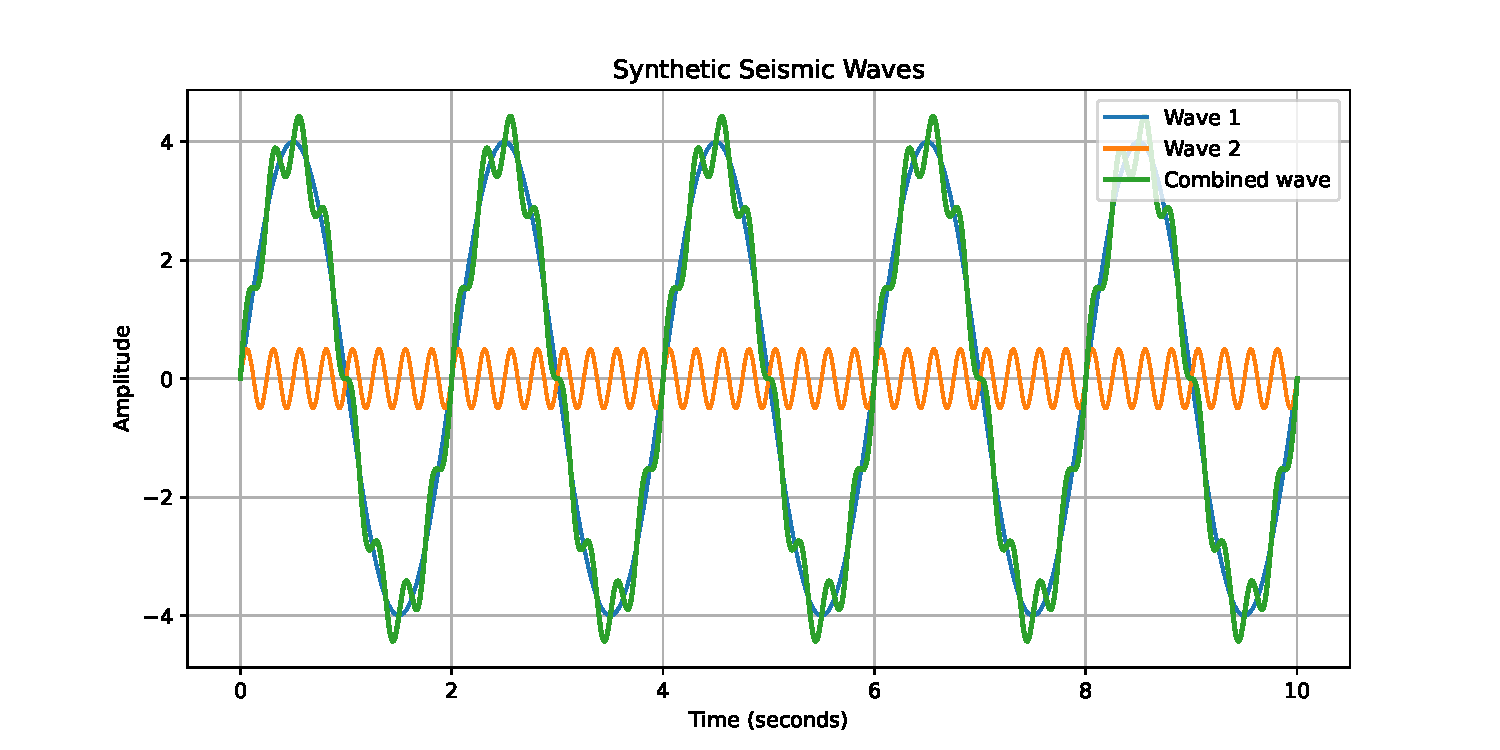
\includegraphics[width=1\textwidth]{sine_waves.pdf}
    \label{fig:sine_waves}
\end{figure}

% ==================================================
% ASSIGNMENT 15
% ==================================================
\assignment{15}{Build Your Own Mountain Range}
{NumPy meshgrid, arrays, 3D plotting}

\begin{missionbox}
You've made it to the final assignment!

Your reward: unlimited mountains.

Use a simple mathematical function
to generate a three-dimensional landscape.

Start with one hill, then add another
to create your own tiny mountain range.
\end{missionbox}

\steps

We'll use the function

\[
z(x,y)=A\exp\left(
-\frac{(x-a)^2+(y-b)^2}{w}
\right).
\]

Here, $A$ controls the hill's height,
$(a,b)$ controls its location,
and $w$ controls its width.

\begin{enumerate}
    \item Create arrays of $x$ and $y$
    coordinates from -10 to 10.
    \item Use \texttt{np.meshgrid()} to
    create a two-dimensional coordinate grid.
    \item Write a function that calculates
    the elevation of a hill.
    \item Evaluate the function over the grid.
    \item Create a 3D surface plot.
    \item Generate a second hill and
    add the two elevation arrays together.
\end{enumerate}

\begin{hintbox}
Create a coordinate grid:

\begin{lstlisting}
import numpy as np

x = np.linspace(-10, 10, 100)
y = np.linspace(-10, 10, 100)

X, Y = np.meshgrid(x, y)
\end{lstlisting}

Evaluate a mathematical function
over the entire grid:

\begin{lstlisting}
Z = 10 * np.exp(-(X**2 + Y**2) / 20)
\end{lstlisting}

Create a 3D plot:

\begin{lstlisting}
import matplotlib.pyplot as plt

fig = plt.figure()
ax = fig.add_subplot(111, projection="3d")

ax.plot_surface(X, Y, Z, cmap="terrain")

ax.set_xlabel("X")
ax.set_ylabel("Y")
ax.set_zlabel("Elevation")

plt.show()
\end{lstlisting}

The \texttt{meshgrid()} function is useful whenever you want to evaluate a function over a two-dimensional domain.
\end{hintbox}

\exampleoutput

Your program should produce a 3D surface containing one or more smooth hills. Try changing the viewing angle, colors, heights, and positions of the hills.

\begin{figure}[H]
    \centering
    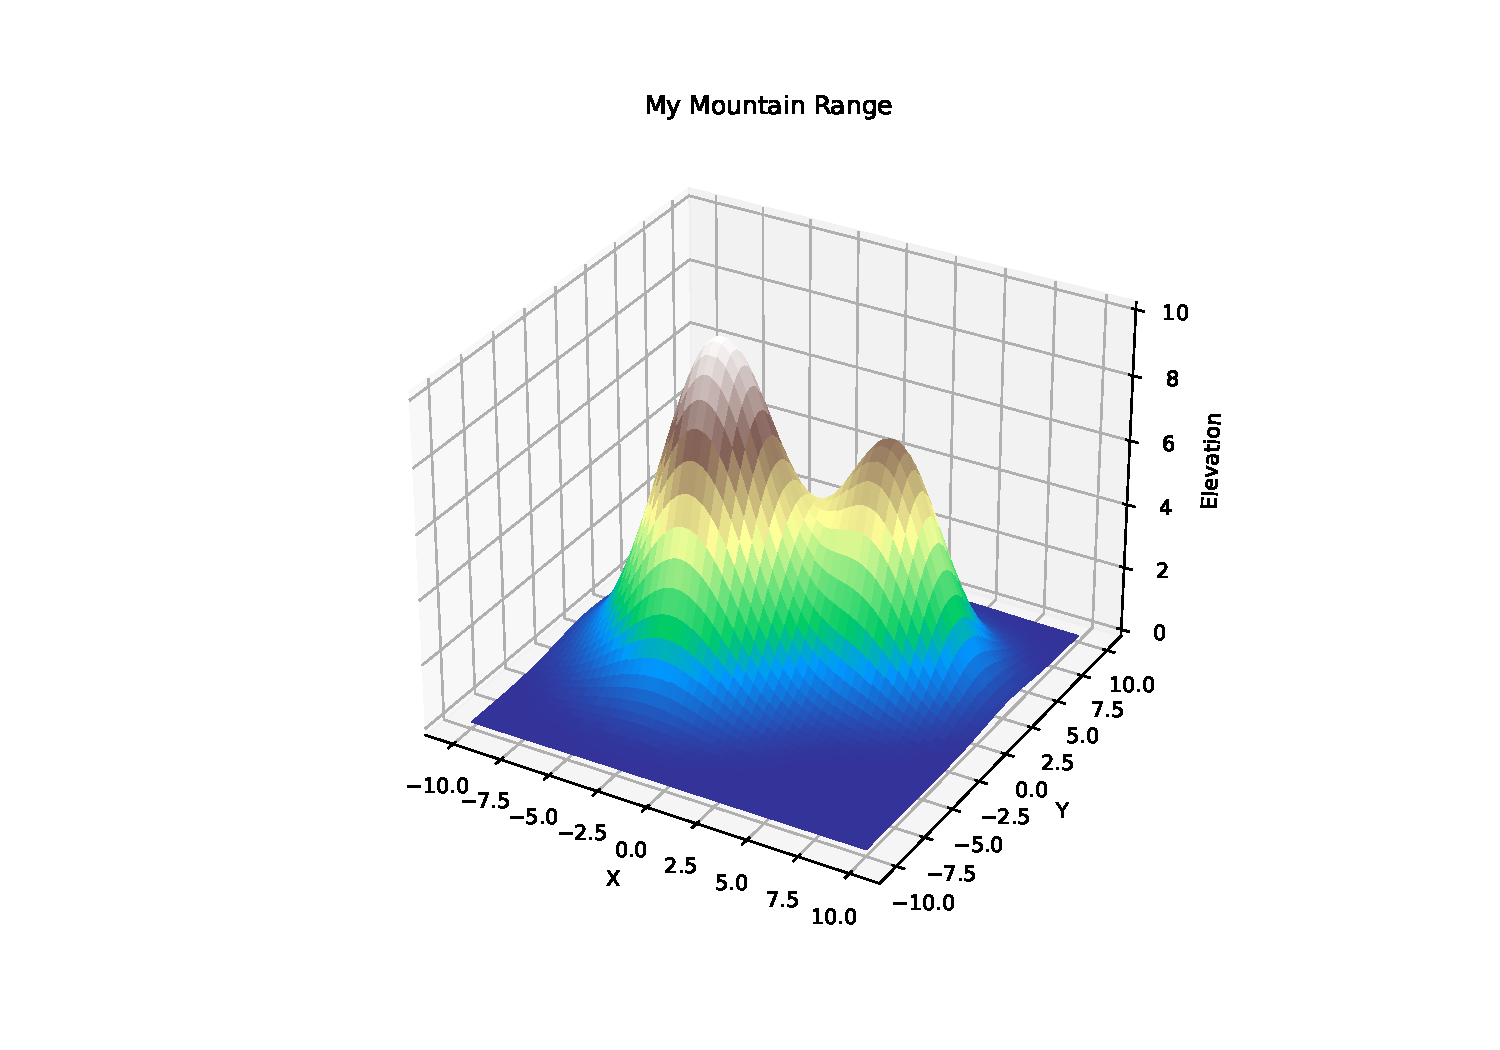
\includegraphics[width=1\textwidth]{mountain_range.pdf}
    \label{fig:mountain_range}
\end{figure}

% ==================================================
% ENDING
% ==================================================
\clearpage

\section*{You Made It!}

Congratulations on completing all 15 assignments!

\begin{center}
\vspace{1cm}
{\Large\bfseries\color{navy}
Happy coding!}
\end{center}

\end{document}
